% The methods that you use goes here
\vspace{0.3cm}
\begin{center}
  \vspace{-0.4cm}
  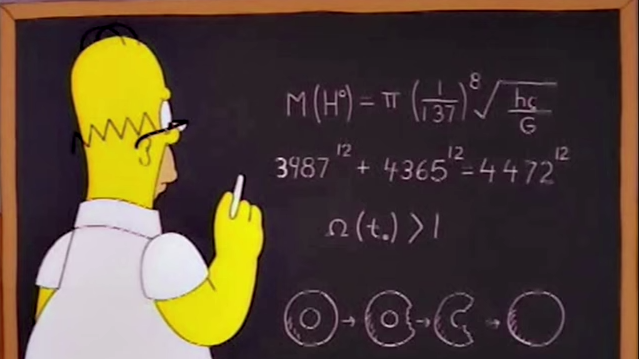
\includegraphics[width=.9\linewidth]{homer_equation}
\end{center}
\vspace{0.25em}
\textsuperscript{[1]}\lipsum[1]
\begin{alignat*}{2}
  u^*(x) := argmin\quad &\mathrlap{\sum_{i=0}^{N-1} l(x_i, u_i) + V_f(X_{N})}&&\\
  \text{subject to}\quad &x_{i+1} &&=\quad f(x_i, u_i),\\
  &g(x_i, u_i)\quad && \le\quad 0\\
  &x_0 &&=\quad x,\\
  &x_N &&\in\quad \mathcal{T}
\end{alignat*}
Lorem ipsum dolor sit amet, consectetuer adipiscing elit. Aenean commodo ligula eget dolor. Aenean massa. Cum sociis natoque penatibus et magnis dis parturient montes, nascetur ridiculus mus. Donec quam felis, ultricies nec, pellentesque eu, pretium quis, sem.
\vspace{2em} % Fill in to put references at the bottom
